\documentclass[11pt]{article}
\usepackage{graphicx}
\graphicspath{ {./pictures/} }

\usepackage[hoptionsi]{subcaption}

%%%%%%%%%%%%%%%%%%%%%%%%%%%%%%%%%%%%%%%%%
% Lachaise Assignment
% Structure Specification File
% Version 1.0 (26/6/2018)
%
% This template originates from:
% http://www.LaTeXTemplates.com
%
% Authors:
% Marion Lachaise & François Févotte
% Vel (vel@LaTeXTemplates.com)
%
% License:
% CC BY-NC-SA 3.0 (http://creativecommons.org/licenses/by-nc-sa/3.0/)
% 
%%%%%%%%%%%%%%%%%%%%%%%%%%%%%%%%%%%%%%%%%

%----------------------------------------------------------------------------------------
%	PACKAGES AND OTHER DOCUMENT CONFIGURATIONS
%----------------------------------------------------------------------------------------

\usepackage{amsmath,amsfonts,stmaryrd,amssymb} % Math packages

\usepackage{enumerate} % Custom item numbers for enumerations

\usepackage[ruled]{algorithm2e} % Algorithms

\usepackage[framemethod=tikz]{mdframed} % Allows defining custom boxed/framed environments

\usepackage{listings} % File listings, with syntax highlighting
\lstset{
	basicstyle=\ttfamily, % Typeset listings in monospace font
}

%----------------------------------------------------------------------------------------
%	DOCUMENT MARGINS
%----------------------------------------------------------------------------------------

\usepackage{geometry} % Required for adjusting page dimensions and margins

\geometry{
	paper=a4paper, % Paper size, change to letterpaper for US letter size
	top=2.5cm, % Top margin
	bottom=3cm, % Bottom margin
	left=2.5cm, % Left margin
	right=2.5cm, % Right margin
	headheight=14pt, % Header height
	footskip=1.5cm, % Space from the bottom margin to the baseline of the footer
	headsep=1.2cm, % Space from the top margin to the baseline of the header
	%showframe, % Uncomment to show how the type block is set on the page
}

%----------------------------------------------------------------------------------------
%	FONTS
%----------------------------------------------------------------------------------------

\usepackage[utf8]{inputenc} % Required for inputting international characters
\usepackage[T1]{fontenc} % Output font encoding for international characters

\usepackage{XCharter} % Use the XCharter fonts

%----------------------------------------------------------------------------------------
%	COMMAND LINE ENVIRONMENT
%----------------------------------------------------------------------------------------

% Usage:
% \begin{commandline}
%	\begin{verbatim}
%		$ ls
%		
%		Applications	Desktop	...
%	\end{verbatim}
% \end{commandline}

\mdfdefinestyle{commandline}{
	leftmargin=10pt,
	rightmargin=10pt,
	innerleftmargin=15pt,
	middlelinecolor=black!50!white,
	middlelinewidth=2pt,
	frametitlerule=false,
	backgroundcolor=black!5!white,
	frametitle={Command Line},
	frametitlefont={\normalfont\sffamily\color{white}\hspace{-1em}},
	frametitlebackgroundcolor=black!50!white,
	nobreak,
}

% Define a custom environment for command-line snapshots
\newenvironment{commandline}{
	\medskip
	\begin{mdframed}[style=commandline]
}{
	\end{mdframed}
	\medskip
}

%----------------------------------------------------------------------------------------
%	FILE CONTENTS ENVIRONMENT
%----------------------------------------------------------------------------------------

% Usage:
% \begin{file}[optional filename, defaults to "File"]
%	File contents, for example, with a listings environment
% \end{file}

\mdfdefinestyle{file}{
	innertopmargin=1.6\baselineskip,
	innerbottommargin=0.8\baselineskip,
	topline=false, bottomline=false,
	leftline=false, rightline=false,
	leftmargin=2cm,
	rightmargin=2cm,
	singleextra={%
		\draw[fill=black!10!white](P)++(0,-1.2em)rectangle(P-|O);
		\node[anchor=north west]
		at(P-|O){\ttfamily\mdfilename};
		%
		\def\l{3em}
		\draw(O-|P)++(-\l,0)--++(\l,\l)--(P)--(P-|O)--(O)--cycle;
		\draw(O-|P)++(-\l,0)--++(0,\l)--++(\l,0);
	},
	nobreak,
}

% Define a custom environment for file contents
\newenvironment{file}[1][File]{ % Set the default filename to "File"
	\medskip
	\newcommand{\mdfilename}{#1}
	\begin{mdframed}[style=file]
}{
	\end{mdframed}
	\medskip
}

%----------------------------------------------------------------------------------------
%	NUMBERED QUESTIONS ENVIRONMENT
%----------------------------------------------------------------------------------------

% Usage:
% \begin{question}[optional title]
%	Question contents
% \end{question}

\mdfdefinestyle{question}{
	innertopmargin=1.2\baselineskip,
	innerbottommargin=0.8\baselineskip,
	roundcorner=5pt,
	nobreak,
	singleextra={%
		\draw(P-|O)node[xshift=1em,anchor=west,fill=white,draw,rounded corners=5pt]{%
		Question \theQuestion\questionTitle};
	},
}

\newcounter{Question} % Stores the current question number that gets iterated with each new question

% Define a custom environment for numbered questions
\newenvironment{question}[1][\unskip]{
	\bigskip
	\stepcounter{Question}
	\newcommand{\questionTitle}{~#1}
	\begin{mdframed}[style=question]
}{
	\end{mdframed}
	\medskip
}

%----------------------------------------------------------------------------------------
%	WARNING TEXT ENVIRONMENT
%----------------------------------------------------------------------------------------

% Usage:
% \begin{warn}[optional title, defaults to "Warning:"]
%	Contents
% \end{warn}

\mdfdefinestyle{warning}{
	topline=false, bottomline=false,
	leftline=false, rightline=false,
	nobreak,
	singleextra={%
		\draw(P-|O)++(-0.5em,0)node(tmp1){};
		\draw(P-|O)++(0.5em,0)node(tmp2){};
		\fill[black,rotate around={45:(P-|O)}](tmp1)rectangle(tmp2);
		\node at(P-|O){\color{white}\scriptsize\bf !};
		\draw[very thick](P-|O)++(0,-1em)--(O);%--(O-|P);
	}
}

% Define a custom environment for warning text
\newenvironment{warn}[1][Warning:]{ % Set the default warning to "Warning:"
	\medskip
	\begin{mdframed}[style=warning]
		\noindent{\textbf{#1}}
}{
	\end{mdframed}
}

%----------------------------------------------------------------------------------------
%	INFORMATION ENVIRONMENT
%----------------------------------------------------------------------------------------

% Usage:
% \begin{info}[optional title, defaults to "Info:"]
% 	contents
% 	\end{info}

\mdfdefinestyle{info}{%
	topline=false, bottomline=false,
	leftline=false, rightline=false,
	nobreak,
	singleextra={%
		\fill[black](P-|O)circle[radius=0.4em];
		\node at(P-|O){\color{white}\scriptsize\bf i};
		\draw[very thick](P-|O)++(0,-0.8em)--(O);%--(O-|P);
	}
}

% Define a custom environment for information
\newenvironment{info}[1][Info:]{ % Set the default title to "Info:"
	\medskip
	\begin{mdframed}[style=info]
		\noindent{\textbf{#1}}
}{
	\end{mdframed}
}
 % Include the file specifying the document structure and custom commands

%----------------------------------------------------------------------------------------
%	ASSIGNMENT INFORMATION
%----------------------------------------------------------------------------------------

\title{Dynamic Distributed Decision Making \\Project 2 \\MIE567} % Title of the assignment

\author{\texttt{Hao Tan 999735728}\\ \texttt{Xiali Wu 999011322} \\ \texttt{David Molina 1005615318}} % Author name and email address

\date{University of Toronto --- \today} % University, school and/or department name(s) and a date

%----------------------------------------------------------------------------------------

\begin{document}

\maketitle

\section{Simulation}
\textbf{In order to implement model-free reinforcement learning algorithms, we need to first have access to a simulator that can recreate the intended behaviours of the environment (MDP) when interacting with it. To do this, create a file called \textit{Gridworld.py} that implements:}
\\

% 1---------------------------------------------------------------
\noindent
\textbf{1.}
\noindent
\textbf{a function that returns the initial state of the MDP: in this case, you
may assume that the initial state is in the bottom right hand corner of the
grid.}

\lstset{language=Python}
\lstset{frame=lines}
\lstset{caption={Returns a random initial state}}
\lstset{label={lst:code_direct}}
\lstset{basicstyle=\footnotesize}
\begin{lstlisting}
def initial_state(self):        # return initial state
    return grid.states[4, 4]
\end{lstlisting}
\\

% 2---------------------------------------------------------------
\noindent
\textbf{2.}
\noindent
\textbf{a function that, given a current state and action, returns the next state and associated reward of arriving at that state.}

\lstset{language=Python}
\lstset{frame=lines}
\lstset{caption={Returns the next state and reward}}
\lstset{label={lst:code_direct}}
\lstset{basicstyle=\footnotesize}
\begin{lstlisting}
def transition_reward(self, current_pos, action): # return the transition probability
    # get next position: state: [0, 0], action: [0, 1], new_state = [0, 1] and reward
    self.new_pos = np.array(current_pos) + np.array(action)
    reward = 0 # normally, reward = 0
    # if new pos results in off the grid, return reward -1
    if -1 in self.new_pos or self.size in self.new_pos:
        reward = -1
    if current_pos == [0, 1]: # if in state A, receive + 10
        reward = 10
    if current_pos == [0, 3]: # if in state B, receive + 5
        reward = 5
    if -1 in self.new_pos or self.size in self.new_pos: # if crossing the border; 
        self.new_pos = current_pos # agent's new_pos is the same as the current pos
    if current_pos == [0, 1]: # if in state A, transition to state A'
        self.new_pos = [4, 1]
    if current_pos == [0, 3]: # if in state B, transition to state B'
        self.new_pos = [2, 3]
    return self.new_pos, reward
\end{lstlisting}
\\
% IMPLEMENTATION-----------------------------------------------
\section{Implementation}
\textbf{Now that you have defined the environment needed to perform
optimization, you are next asked to implement four of the standard reinforcement
learning algorithms you have learned in this course so far. This includes:}\\

\\
\indent\textbf{1. First-Visit On-Policy Monte Carlo for Control}
\\
\indent\textbf{2. Q-learning}
\\
\indent\textbf{3. SARSA}
\\
\indent\textbf{4. SARSA$(\lambda)$ using eligibility traces}
\\

\noindent
\textbf{Each algorithm should be implemented in a separate Python file and be
named appropriately (MonteCarlo.py, QLearning.py, Sarsa.py and SARSALambda.py).
For each algorithm you implement, you should have another Python file that
allows to run your experiment.} \\

\noindent
We initialize our domain, and the algorithm with following parameter settings. We applied the same parameter settings for each of the four algorithms. We fix the episode length to 200 and the total number of episodes to 500.  We initialize your Q-values to zero. Please refer to the algorithm files.

\begin{equation}
\gamma = 0.99
\end{equation}
\begin{equation}
\lambda = 0.9
\end{equation}
\begin{equation}
\alpha = 0.1
\end{equation}
\begin{equation}
\epsilon \in\{0.01,0.1,0.25\}
\end{equation}\\

\noindent
\textbf{In order to get a better idea of how fast each algorithm converges,
practitioners typically run each algorithm independently using the same initial
conditions many times (run each one at least 20 times), and average the results
from all the trials.} \\

\noindent
\textbf{Plotting the performance of each algorithm and each ε combination, you
may plot the mean over all trials (you don’t have to plot each individual
trial).} \\

\noindent
\textbf{For each experiment, you are responsible for reporting (these can be
reported as averages of many trials, as mentioned above):} \\

\noindent
\textbf{• at the end of each episode of training, you should test the
performance of the greedy policy with respect to your learned Q-values (the
policy that chooses actions in argmaxQ(s, a)} \\

\noindent
\textbf{• you must include a plot of both training performance and test
performance for each experiment: you can measure the performance during an
episode by the average, total or discounted return you obtained by running that
policy} \\

\noindent
\textbf{• you should report the final Q-values you obtained for each experiment
and the policy you obtained on a typical run: if you obtained different policies
or performance, report several typical results you observed}


% COMPARISON & WRITE_UP-------------------------------
\newpage
\section{Comparison and Write-up}
\textbf{1.For each algorithm, what was the best and worst values of $\epsilon$
(in terms of test performance)? How different is the train and test performance
between algorithms for each value of $\epsilon$? How different is the train and
test performance between values of $\epsilon$ for each algorithm (e.g. how
sensitive was each algorithm to $\epsilon$)? Why do you think this occurred?
Does this coincide with what you learned in lectures about each algorithm?} \\
\noindent
xxx
\\
\textbf{2.What was the final policy and Q-values that you typically obtain (typically, as in the
majority of the trials)? Are they similar or different across algorithms for each value
of ε? Does this correspond to an optimal policy (you may refer to your answers for
project 1)? Please comment on the variability of each algorithm in terms of what
you learned about the algorithms (e.g. bias/variance trade-off).}
\\
\noindent
xxx
\\
\textbf{3.Which algorithm was most difficult, and which was most easy, to
implement and why? Which took the least time (and samples) to train, and which
the most? Which algorithm(s) do you think would scale better to larger problems
and why?} \\
\noindent
xxx
\\

% APPENDIX-------------------------------------
\newpage
\section{Appendix}

% \begin{figure}[h]
% 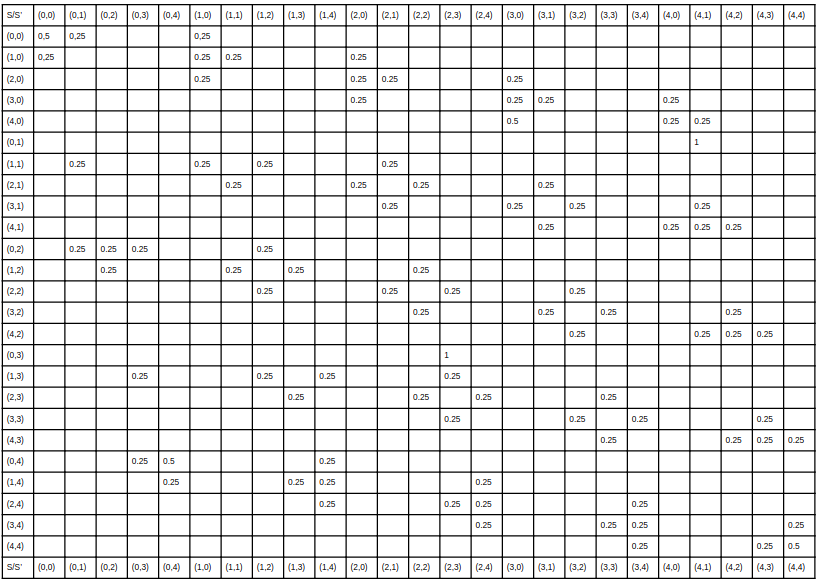
\includegraphics[scale=0.5]{transition_matrix}
% \centering
% \caption{Transition Matrix}
% \end{figure}

\end{document}
